\subsection{Функция Гаусса}

Рассмотрим семейство функций
\begin{equation}
    f(t) = a e^{-bt^2}
    \label{eq:gaussian_function}
\end{equation}

\subsubsection{Графики исходных функций}
Графики данной функции при различных значениях $a$ и $b$ представлены на рисунках \ref{fig:gaussian_1}, \ref{fig:gaussian_2} и \ref{fig:gaussian_3}.

\begin{figure}[ht!]
    \centering
    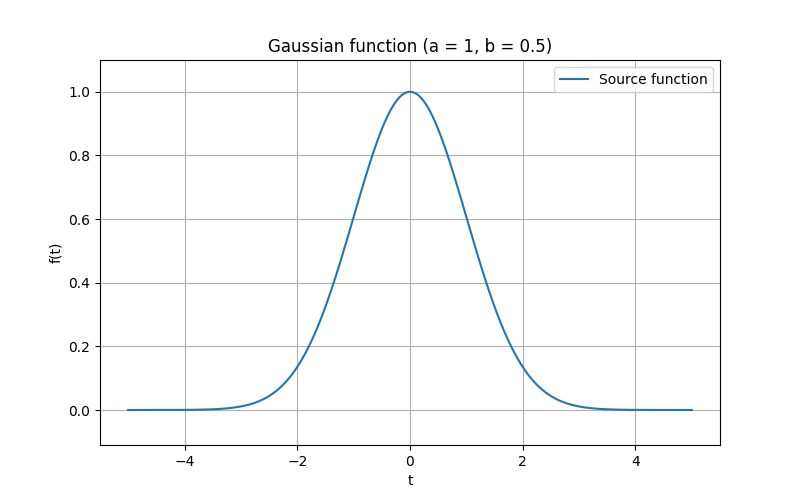
\includegraphics[width=\textwidth]{media/gaussian_1.png}
    \caption{График функции $f(t)$ при $a = 1$, $b = 0.5$}
    \label{fig:gaussian_1}
\end{figure}

\begin{figure}[ht!]
    \centering
    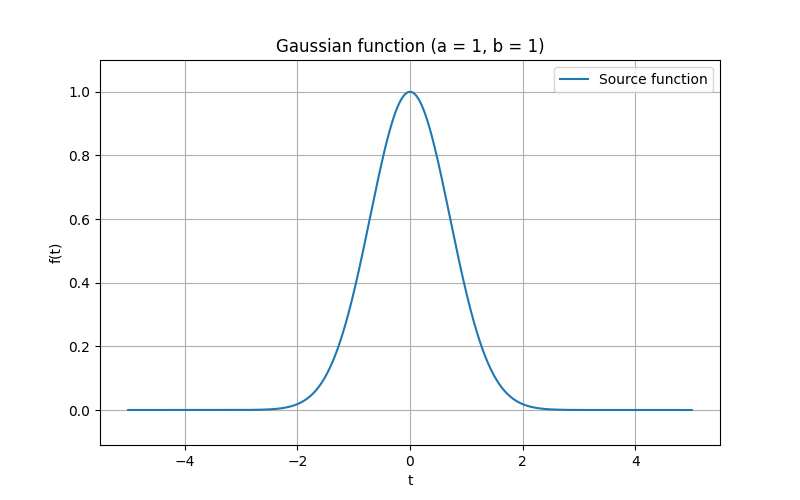
\includegraphics[width=\textwidth]{media/gaussian_2.png}
    \caption{График функции $f(t)$ при $a = 1$, $b = 1$}
    \label{fig:gaussian_2}
\end{figure}

\begin{figure}[ht!]
    \centering
    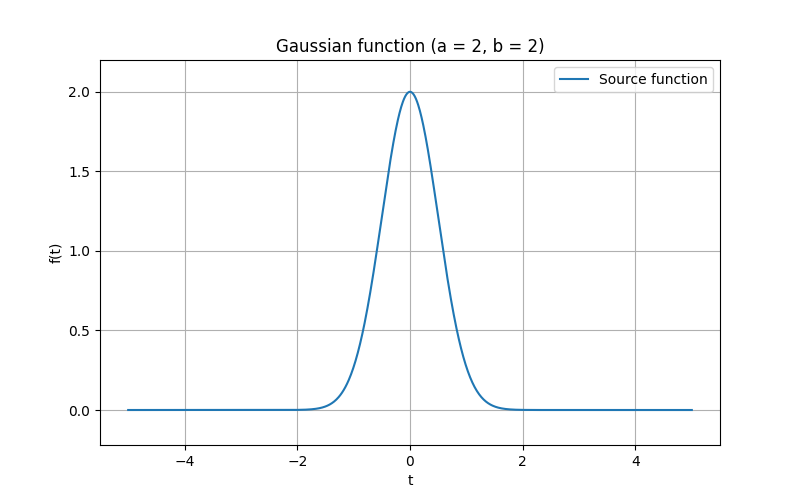
\includegraphics[width=\textwidth]{media/gaussian_3.png}
    \caption{График функции $f(t)$ при $a = 2$, $b = 2$}
    \label{fig:gaussian_3}
\end{figure}

\subsubsection{Нахождение образа функции}
Согласно формуле \eqref{eq:image_from_function}, Фурье образ функции $f(t)$ задается следующим выражением:
\begin{multline}
    \hat{f}(\omega) = \frac{1}{\sqrt{2\pi}} \int_{-\infty}^{\infty} f(t) e^{-i\omega t} dt = \frac{1}{\sqrt{2\pi}} \int_{-\infty}^{\infty} a e^{-bt^2} e^{-i\omega t} dt = \frac{a}{\sqrt{2\pi}} \int_{-\infty}^{\infty} e^{-bt^2} e^{-i\omega t} dt = \\
    \frac{a}{\sqrt{2\pi}} \int_{-\infty}^{\infty} e^{-t(bt +i\omega)} dt = \frac{ae^{\frac{-\omega^2}{4b}}}{\sqrt{2b}}
\end{multline}

\subsubsection{Графики образов функций}
Графики образов функции \eqref{eq:gaussian_function} при различных значениях $a$ и $b$ представлены на рисунках \ref{fig:gaussian_1_image}, \ref{fig:gaussian_2_image} и \ref{fig:gaussian_3_image}.

\begin{figure}[ht!]
    \centering
    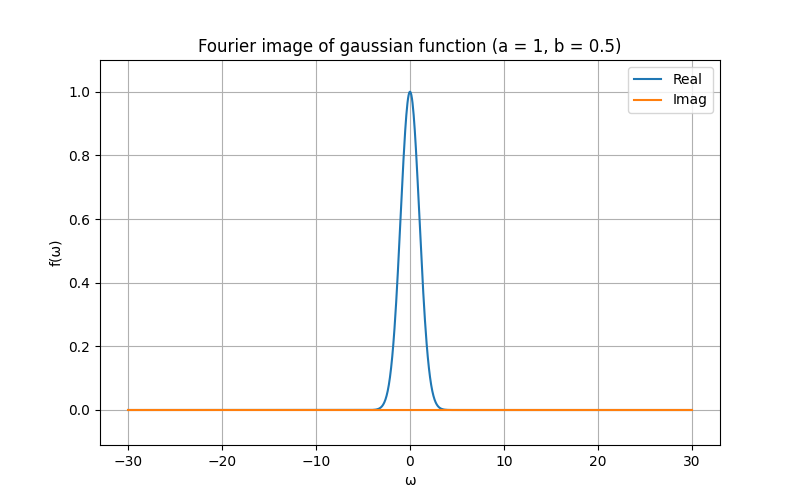
\includegraphics[width=\textwidth]{media/gaussian_1_image.png}
    \caption{График образа функции $f(t)$ при $a = 1$, $b = 0.5$}
    \label{fig:gaussian_1_image}
\end{figure}

\begin{figure}[ht!]
    \centering
    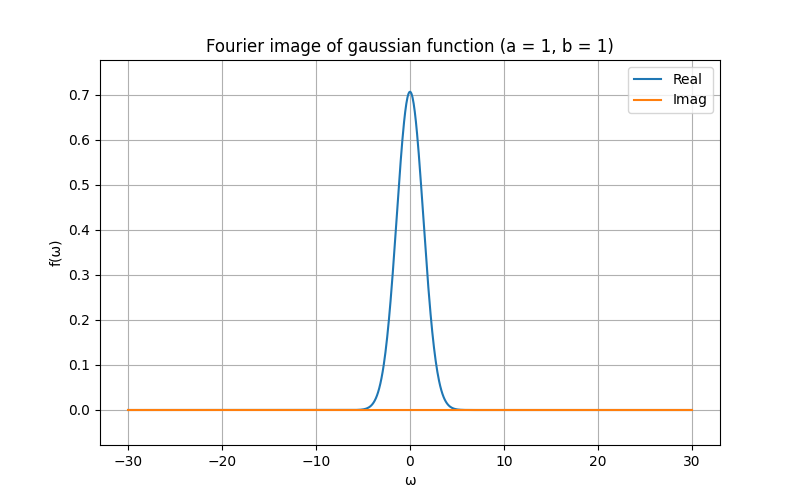
\includegraphics[width=\textwidth]{media/gaussian_2_image.png}
    \caption{График образа функции $f(t)$ при $a = 1$, $b = 1$}
    \label{fig:gaussian_2_image}
\end{figure}

\begin{figure}[ht!]
    \centering
    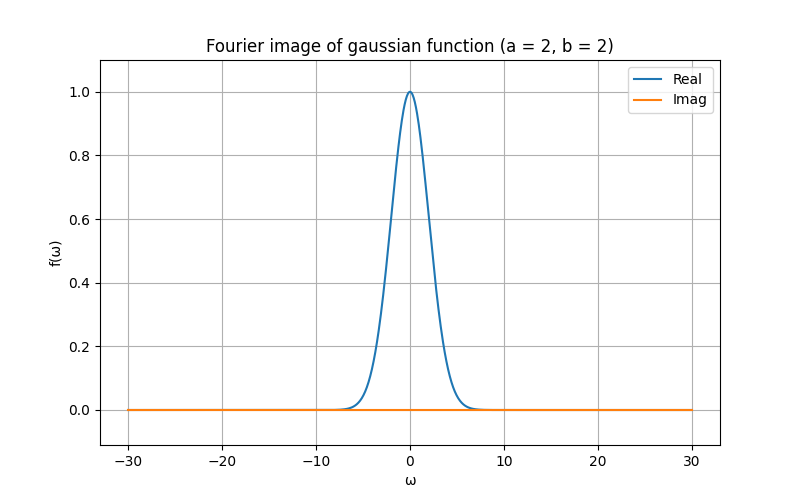
\includegraphics[width=\textwidth]{media/gaussian_3_image.png}
    \caption{График образа функции $f(t)$ при $a = 2$, $b = 2$}
    \label{fig:gaussian_3_image}
\end{figure}

\FloatBarrier
\subsubsection{Провека равенства Парсеваля}
Проверим выполнение равенства Парсеваля для функции \eqref{eq:gaussian_function} при $a = 1$, $b = 1$:
% table with parseval check results
\begin{table}[ht!]
    \centering
    \begin{tabular}{|c|c|}
        \hline
        $\displaystyle\int_{-100}^{100}{|f(t)|^2}$ & $\displaystyle\int_{-100}^{100}{|\hat{f_1}(\omega)|^2}$ \\
        \hline
        1.7724 & 1.7724 \\
        \hline
    \end{tabular}
    \caption{Результаты проверки равенства Парсеваля для функции Гаусса $f(t)$ при $a = 1$, $b = 0.5$}
    \label{tab:gaussian_1_parseval_check}
\end{table}

\begin{table}
    \centering
    \begin{tabular}{|c|c|}
        \hline
        $\displaystyle\int_{-100}^{100}{|f(t)|^2}$ & $\displaystyle\int_{-100}^{100}{|\hat{f_2}(\omega)|^2}$ \\
        \hline
        1.2533 & 1.2533 \\
        \hline
    \end{tabular}
    \caption{Результаты проверки равенства Парсеваля для функции Гаусса $f(t)$ при $a = 1$, $b = 1$}
    \label{tab:gaussian_2_parseval_check}
\end{table}

\begin{table}
    \centering
    \begin{tabular}{|c|c|}
        \hline
        $\displaystyle\int_{-100}^{100}{|f(t)|^2}$ & $\displaystyle\int_{-100}^{100}{|\hat{f_3}(\omega)|^2}$ \\
        \hline
        3.5449 & 3.5449 \\
        \hline
    \end{tabular}
    \caption{Результаты проверки равенства Парсеваля для функции Гаусса $f(t)$ при $a = 2$, $b = 2$}
    \label{tab:gaussian_3_parseval_check}
\end{table}

Видим, что равенство Парсеваля выполняется для всех значений $a$ и $b$ с точностью до способа вычисления интегралов.

\subsubsection{Анализ результатов}
Влияние параметров $a$ и $b$ на функцию Гаусса можно понять по формулам \eqref{eq:gaussian_function} и \eqref{eq:image_from_function}. Параметр $a$ отвечает за амплитуду функции, а параметр $b$ за ширину исходной функция. При увеличении $a$ амплитуда функции увеличивается, при увеличении $b$ функция становится уже. 
Эти выводы подтверждаются графиками исходной функции и ее образа.

Данная функция является единственной из рассмотренных, у которой образ может быть в точности равен исходной функции. 

\begin{equation}
    ae^{-bt^2} = \frac{ae^{\frac{-\omega^2}{4b}}}{\sqrt{2b}}
\end{equation}

Решив это уравнение, получим корни $a - \text{любое}$, $b = \frac{1}{2}$. Таким образом, при данных параметрах образ функции Гаусса будет равен исходной функции.